\chapter{Methodology}
When developing technology systems it is important to involve the user in the process to make something that fits the users needs and wants. Data collection is a key role to gather information about the users needs and to establish requirements to the systems. The primary methods used in this thesis are experimental simulation, and qualitative research methods like participatory observation and focus group interviews. In addition, support methods like video and audio recording, and a survey are used. The latter was used to in an efficient way gather information about  who the informants were, and their attitudes towards exercising and technology in general. We arranged two sessions, which we have called workshops.  The definition of a workshop is "A meeting at which a group of people engage in intensive discussion and activity on a particular subject or project" \cite{dictionary}. This definition fits well with both our sessions. Workshop 1 was organized as an experimental simulation, as defined by McGrath \cite{McGrath}. We invited a group of relevant users to participate in a setting that we tried to make as natural as possible. Experimental simulation will be described in more detail in Section \ref{sec:experimental} The execution of workshop 1 will be described closer in Section \ref{sec:ws1}. Based on the findings from workshop 1, in addition to findings done in the literature, we developed requirements for a video game concept, and made low-cost/low-fi prototypes. This concept was presented by the use of prototypes, story telling and acting, for a potential user group. The users were engaged to discuss the concept in a focus group. This session is described as workshop 2.

In the first part of this chapter we will give an overview of the importance of user involvement, and the relevant research strategies and methodologies used in this thesis to meet the requirements of user involvement. We will also discuss ethical challenges and the different criteria for the quality of the research. At the end of this chapter we will give a thorough presentation of the execution of the two workshops conducted in this thesis. 

\section{User Involvement}
\label{sec:userinvolvement}
There is no definitive solution on how to make a good and user friendly system, and it is challenging and time consuming to find the users needs. For a system design to experience success interaction designers have to pay attention to various aspects of the user. The best way to do this is to involve users in the process of developing the system, from requirement definition and the design phase, to prototype and system test, all to the end of the system's life cycle \cite{mmi}. ISO 13407 presents activities included in the cycle of user centered design, which is shown in Figure \ref{userdesign}. ISO 9241-210 describes why it is important to include users in system development \cite{dis20109241}:

\emph{"Involving users in design and development provides a valuable source of knowledge about the context of use, the tasks, and how users are likely to work with the future product, system or service. User involvement should be active, whether by participating in design, acting as source of relevant data or evaluation situations [...]"}

\begin{figure} [H]
\centering
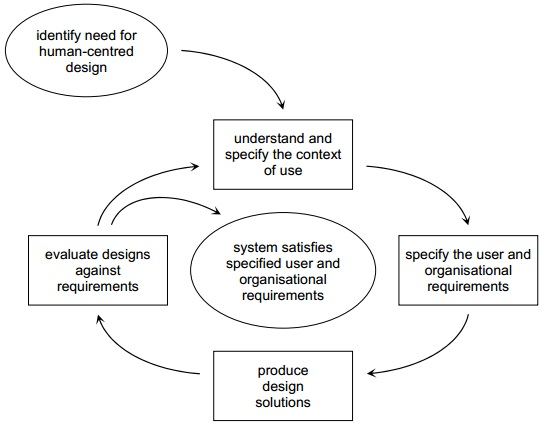
\includegraphics[scale=0.7]{userCenteredDesign.jpg}
\caption[User centered design]{Activities of user centered design, from ISO 13407 \cite{jokela2003standard}}
\label{userdesign}
\end{figure}

User involvement focus on finding future users of the system to be made, and let them take part in decision making during the development process \cite{bjerknes1995user}. User involvement provides the opportunity for developers and future users to meet and discuss topics and issues related to the system. This gives the users knowledge about system features and functionality, and it makes it possible for developers to get to know and understand their potential users. Participation in the development process will give users the possibility to influence how the final system will be. This could lead to a feeling of ownership, which again will increase the probability for users to accept and employ the final system. User involvement will also increase the probability for developers to make good and user-friendly interfaces \cite{infodesign} \cite{mmi}. 

When creating something completely new, it is all about understanding what the users want and need, but often the users themselves do not know what they want. It will not be possible to walk up to a potential customer and ask what he or she wants and needs. This does not mean that a developer should be creative, come up with a great idea and bring it into life without ever talking to the user group. The development of a new system should be done as a cyclic process, where development and user involvement goes hand in hand \cite{mmi}.  

The importance of user feedback throughout the development process is stated in ISO 9241-210 \cite{dis20109241}:

\emph{"Feedback from the users is a critical source of information in human-centered design. Evaluation designs with users and improving them based on their feedback provides an effective means of minimizing the risk of a system not meeting user or organizational needs (including those requirements that are difficult to specify explicitly).  [...] User-centered evaluation should also take place as part of the final acceptance of the product to confirm the requirements have been met. Feedback from users during operational use of identifies long-term issues and provides input to future design."}

\subsection{Use of Prototypes}
\label{sec:prototypes}
We have now presented the usefulness of involving users in a system's development process, where the users is involved all the way from the start to the end. What might be difficult in the early stages of system development is to, in a realistic way, present for the users how the final system will look like. If the users starts of getting a wrong impression of the final system, this may lead to situations where the system design is finished and the users are left with the feeling of not being satisfied. This would be a problem, because of the high costs associated to making changes in the already implemented system. Trying to avoid situations like this, designers introduce use of prototypes. 

Prototyping is a method used to evaluate, explore and express functionality and system design \cite{houde1997prototypes}. Prototypes is defined in \cite{mackayprototyping} as \emph{"a concrete representation of part or all of an interactive system. A prototype is a tangible artifact, not an abstract description that requires interpretation. Designers, as well as managers, developers, customer and end-users, can use these artifacts to envision and reflect upon the final system"}. Use of prototypes is helpful for designers in terms of creating and presenting ideas in a realistic way, and to get feedback from users on what they have created. Prototypes is also helpful when designers has to choose between various design alternatives. They make is easy to express, and to reflect over, ideas, and they support creativity among all people, regardless of their experience with technology. They also communicate functionality and system design between designers and the users and customers, which makes it possible to evaluate the system early in the development process \cite{mackayprototyping} \cite{mmi}. \emph{"Prototypes reveals the strengths as well as weaknesses of a design. Unlike pure ideas, abstract models or other representations, they can be contextualized to help understand how the real system would be used in a real setting"} \cite{mackayprototyping}. Not only makes prototypes it possible for designers to get feedback from users, but is also helps them analysing users needs due to system functionality. 

There are several ways to make prototypes, from simple sketches on paper, to up-and-running software systems. How designers talk about prototypes is dependent on how the prototypes look according to final design, and what kind of tools that have been used to make them.  Designers distinguish between low- and high-fidelity prototypes \cite{mackayprototyping} \cite{houde1997prototypes} \cite{mmi}, where "fidelity" refers to how close the prototype is to the final design. Low-fidelity (lo-fi) prototypes usually is a presentation of design concepts on paper \cite{mmi} \cite{lofihifi}. They can be related to what is called off-line prototypes, which is prototypes that does not run on a computer. Normally these are paper sketches, story-boards, and mock-ups. Advantages with use of lo-fi prototypes are that they promote creativity, and that they are fast, cheap and easy to make and change. Lo-fi prototypes could also be presented as low-tech because no implementation is needed to make them \cite{lofihifi}. No software system are used to make these prototypes, which makes it possible for all sort of people to take part in the design, as no programming knowledge are required. High-fidelity (hi-fi) prototypes often present the final result in a more realistic way than lo-fi prototypes \cite{mmi}. These can be related to what is called on-line prototypes, or "software prototypes", which are prototypes that are computer dependent. This could be videos, programmed systems, animations, or applications made with various design tools \cite{mackayprototyping}. Hi-fi prototypes can be referred to as high-tech because they include partial or finished implementation of functionality. What is negative with these prototypes is that they require more time, cost and knowledge to be made, and that the use of various programming languages or development tools could restrain creativity. This could be due to problems developing a specific design idea, and that the use of these tool excludes involvement of users with no programming knowledge.    

In addition to lo-fi and hi-fi prototypes, there are horizontal and vertical prototypes. With horizontal prototypes a wide range of functionality are shown, without the underlying functionality implemented. This gives an overall presentation of the functionality and design from the users point of view. With vertical prototypes, fewer functions are shown, but in return, these functions are implemented. These prototypes will usually show functionality from the system level \cite{mackayprototyping} \cite{horver}.

\emph{"An important characteristic of HCI systems is that they are interactive: users both respond to them and act upon them"} \cite{mackayprototyping}. Interactive systems can be complex, and it can therefore also be difficult to design prototypes that shall present these systems. In addition, when designing a prototype, the designer has to think of how the user can interact with it. How the prototypes are presented to the users plays is critical on how they will understand the system. There can be designed prototypes that the user will not be able to interact with, or pretend to interact with. These are usually used to present scenarios. There can also be made prototypes, both paper prototypes and software prototypes, that users can interact with. In between these situations, there is something called the "Wizard of Oz". Here one person will control or act as the interactive system, while another person are in the role as the user. Which method used to present the prototype is not the main issue, what is most important is that the users \emph{feel} that they are interacting with the system.

When the designer is about to develop prototypes, it is important to take into consideration the role and purpose of the prototype. The choice of prototype development, and presentation of the prototype, has to be made according to the  purpose the designer has with presenting them to the users \cite{mackayprototyping}. The choice of focus for the prototype is highly important to be able to identify crucial design questions. Houde et al. presents in \cite{houde1997prototypes} a model that says something about what prototypes prototype. This takes the systems role, implementation, and look and feel into consideration. Implementation as about the technique and components used in the system. The role is about the systems function in the users lives. Look and feel involves the users experience and perception of the system, like what the users can feel, see and hear. This will simulate the look of the system, without including the actual purpose of the system. The model is presented in Figure \ref{fig:prototype} a). Placing the prototype in this figure will describe what the prototype it meant to explore \cite{houde1997prototypes}.    

We have developed prototypes to be able to present our idea for a video game concept. The prototypes are horizontal, showing all functionality and information that will be in the game, but they are not implemented such that interaction with them are possible. They only present the various functionality and scenarios from the video game concept. Our prototypes are hi-fi in terms of being developed with software drawing tools like Photoshop, and that they are realistic due to final interface design. However, they are lo-fi due to the technology implemented (which is none). We will therefore describe our prototypes as medium-fidelity, including "the best from both worlds". When presenting our video game concept we showed the various prototypes and described what happened in the prototype. There was no interaction between the prototypes and the users. However, one of us stood in front of the prototype, simulating the movement of the avatar on the screen, trying to show interaction. In addition to the scenarios, we prototyped a menu with the use of PowerPoint. The menu was presented with the "Wizard of Oz" technique, with one controlling the PowerPoint presentation, while the other acted as the users and simulated pressing buttons and reviewing the menu. In Figure \ref{fig:prototype} b) we have placed our prototypes within the prototype model. Our prototypes are represented by a red circle by the corner that represent look and feel. This is because we wanted to get feedback on the experience of our video game concept. The circle is directed a bit towards the role of the prototype, as we also had focus on where the final system would be used. 

\begin{figure} [H]
\centering
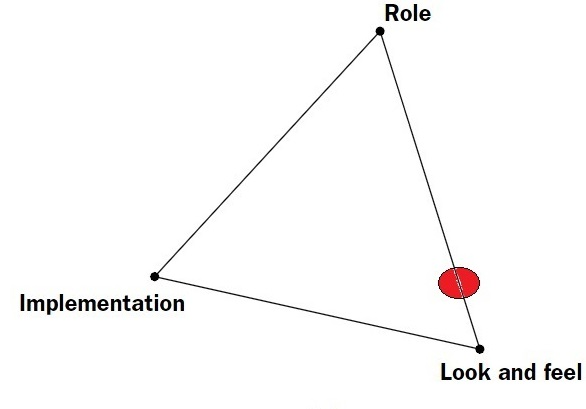
\includegraphics[scale=0.4]{prototypemodelDobbel.jpg}
\caption[Prototype model]{A model of what prototypes prototype, \cite{houde1997prototypes}. Figure a) shows the general model, and figure b) shows the placement of our prototypes.}
\label{fig:prototype}
\end{figure}

\section{Choosing the Setting for Our Study}
\label{sec:experimental}
When doing research there are three criteria you would like to maximize \cite{McGrath}, \cite{alsos}: 

\begin{itemize}
\item Generalizability of the evidence,
\item Precision of measurements, and 
\item Realism of the study context.  
\end{itemize}

However, it is not possible  to maximize all three criteria because if you do something to increase one criteria, you are likely to decrease an other criteria. In our study realism is the most important criteria and is the one we want to maximize as much as possible.

There are different research strategies that can be used. Sometimes it is hard to find one that fits exactly to what you as a researcher want to do.
\begin{figure}
\begin{center}
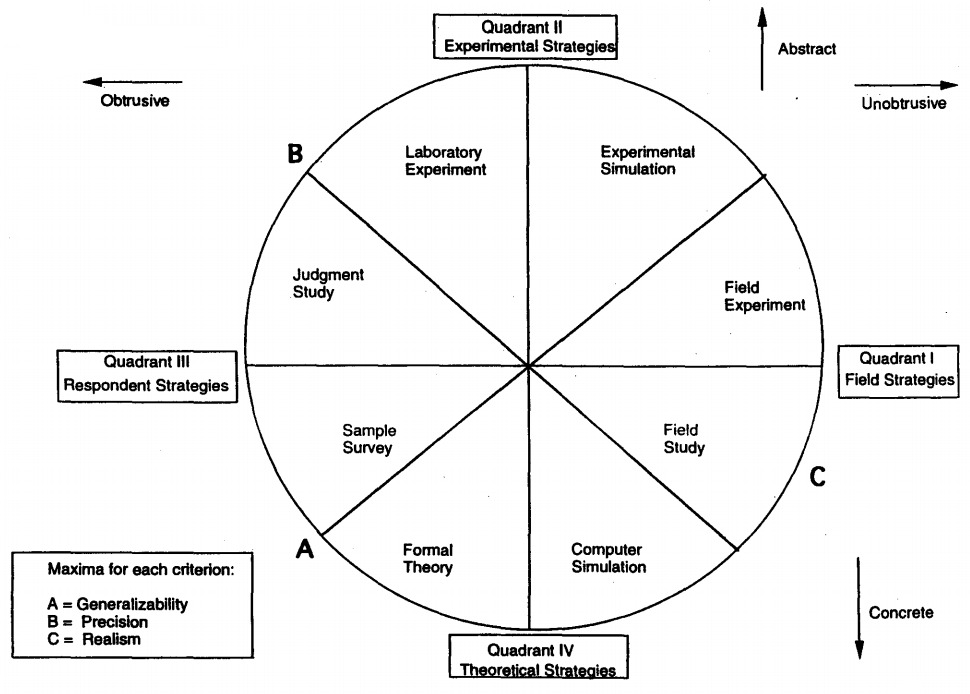
\includegraphics[scale=0.5]{circumplex}
\caption[The strategy circumplex]{The strategy circumplex (modifid by \cite{alsos} from \cite{McGrath})}
\label{fig:circumplex}
\end{center}
\end{figure} 
The strategy circumplex by McGrath is shown in Figure \ref{fig:circumplex}. This figure presents eight different strategies \cite{McGrath}. As can be seen from the figure the different strategies are arranged in a way on whether they are abstract versus concrete, and obtrusive versus unobtrusive. The figure also shows at what strategy the three different criteria, generalizability, precision and realism, are at their maximum. We studied this circumplex to find where our study fits in. We found one of the strategies from quadrant 2 appropriate. Within this quadrant there are two different strategies, laboratory experiment and experimental simulation. In the former strategy the researcher put together a setting and invite some individuals to enter the setting and act by the defined rules. Here the researchers typically know what behaviour they are looking for and can within this setting study this with precision. The second strategy is experimental simulation. At the same time as trying to get the precision, as in a laboratory experiment, the researcher also try to get some more realism than the strategies in quadrant 3 do. This means that the researchers are setting up a situation like in the laboratory experiment, but at the same time are trying to get some realistic behaviours from the participants. This means that the researchers try to get sufficient realism, and at the same time keeping precision and control. The field experiment strategy within quadrant 3 was also considered because we found it in some ways to fit for our study. This strategy, compared to field study which has maximum degree of realism, opens up for being a little more obtrusive, and in that way give up some of the realism. We wanted to create an as natural setting as possible, and to implement the study in a place familiar to the informants. However, as defined in \cite{McGrath}:  \emph{"The essence of both of the strategies in quadrant 1 [shown as 3 in this figure], the field study and the field experiment, is that the behaviour system under study is "natural", in the sense that it would occur whether or not the researcher were there and whether or not it were being observed as part of a study"}. In contrast, the behaviour gotten from the two strategies within quadrant 2, would not have been apparent if it was not for the researchers doing the study, which is the case in our study. Therefore, we conclude that we in our study uses some variant of experimental simulation, even though no study is fully under only one strategy. It is important to understand that even though experimental simulation is less realistic, the study is still real and the behaviours gotten from the participants are real, however influenced by the setting \cite{McGrath}. Because the experimental simulation never can be as realistic as the field study, there will be an error in the information gathering, which can pose validity issues \cite{alsos}. The validity of our research will be discussed in more detail in Chapter \ref{chap:discussion}. We will now discuss research methods used to gather data from the experimental simulation. 


\section{Qualitative Research}
Qualitative research is a method used to get an in-depth understanding of a phenomenon. This research method is well suited when studying sensitive and personal topics, as well as when studying topics that there have not been done much research on. Interpretation is very important in qualitative methods, as well as flexibility and openness. With flexibility it means that the scheme should have the possibility to be changed during the research, if needed. The focus in this research method lies on how and why things are done, and not how many who does it, like in quantitative methods. Quantitative methods include huge samples, while qualitative research can give more information about a small sample \cite{qualitative}. This often result in a close and personal relationship with the people being studied \cite{tjora}.  \\ \\
The qualitative research process can be divided into phases, that partially overlap. The first phase consists of defining what the research will find out. We have done this be defining some research questions which can be found in Chapter 2. The next phase is the data gathering phase. This phase can be performed with several methods. The following phase includes interpreting and analysing of the data, as well as formulating theories. In the last phase, the results will be presented. Data gathering and analysis should be done in parallel. In that way, further data gathering can be adjusted from what have found in earlier analysis. There are four different data gathering methods described by Thagaard in \cite{qualitative}:

- Observation \\
- Interview \\ 
- Document analysis, and \\
- Analysing of video and audio recordings

The most common methods are interviews and participatory observation. These are primarily the two methods we have used in our thesis. It is common in qualitative research to have a close connection between the researcher and the people who is being studied. This especially apply in interviews and observation. This contact is important for the data the researcher will gain from the study \cite{qualitative}. The interview method and the observation method will be described in more detail later in this section.

In most qualitative methods it is common to textually document the data which is being analysed. The documentation can include what people do, their statements, their intentions or their perspectives. The text can be notes from the field or printouts of  recorded interviews \cite{qualitative}. In this thesis we have textually transcribed video and audio recording, and used  \ac{sdi} to analyse this data. This will be discussed later in this section.

\subsection{Ethical Challenges}
The close contact established between the researcher and the informants introduces some ethical challenges. All results conducted from the research needs to be precisely and correct when presented. This also includes other researcher's work. Plagiarizing means to copy other people’s work and take credit for it. This is illegal, and it is therefore important to properly state the resource of the information that is being presented.  When working in close contact with informants, the researcher often gets personal information about the informants. Personal information means information that can be linked to individuals. In projects with this kind of information, the project needs to be reported. In the case of research projects performed at universities, the project needs to be reported to \ac{nsd}, which is an entity in care of data protection for these institutions. \ac{nsd} will evaluate each project in accordance to research ethical rules \cite{qualitative}. In this thesis we will do observation of a fixed workshop, as well as focus group interviews with the participants of the workshop. This will require having a close connection with the participants, as well as gather personal information about them. In addition, we will video record the workshop and audio record the interviews. Therefore, this thesis has been reported to \ac{nsd}, see Appendix X. 

\subsubsection{Ethical Guidelines:}
Tjora \cite{tjora} suggests that common politeness should be a basis for ethical research. However, some additional rules needs to be followed. These are described in the following guidelines:

\emph{Informed Consent:} \\
In a research project with people involved, there is a requirement that the researcher has the participant's informed consent. This means that the informants have gotten all the information they need to know about the participation, have self chosen to participate, and that they can withdraw at any time without any consequences. One challenge about this, is that in some projects too much information can affect the participants behaviour (for example if the participants know too much about what the researchers are looking for, they can act differently) \cite{qualitative}. Because of the setting of our workshop we did not see this as a problem for our research, so the participants were well informed on what we were researching. To get participants to our study we held a presentation for a group of relevant people, where we described the project and the workshop. In addition, all participants, got an invitation letter, with a short description of the project and information about what they were going to participate in, and their rights. Every participant gave us their written consent to participate. The presentation, invitation and written consent can be found in Appendix Y.   \\ \\
\emph{Confidentiality:}\\
Researchers are required to keep all the information they collect about a participant confident. This means that the information have to be anonymized. This also involves strict requirements to how personal data, that makes it possible to identify individuals, should be stored and annulled. There are rules about how long data can be stored. General principles are that data should be stored for only the amount of time there is use for the data, and that data which can be directly linked to an individual should be stored separately and not electronically.  Reuse of data is not allowed without consent from the participants \cite{qualitative}. In this thesis we have signed a non-disclosure agreement to assure the participant that we will not reveal any confident information about them. This is found in appendix Z. In addition, we have assured the participant that all data we collect will be deleted within 3 years after the project's end. See Appendix Y. \\ \\
\emph{Consequences of participating in research projects:}\\
The researcher has responsibility over the participants safety and should respect their wishes. It is important to have thought through what consequences the execution of the research may have for the participants. The researcher is required to protect the participant's integrity during the process \cite{qualitative}. In our workshop, all participants were allowed to choose what they were comfortable with doing and not doing. They were allowed to withdraw at any time without any consequences.  \\ \\

\subsection{Observation}
Observation, often called ethnography \cite{tjora}, is used when the researcher wants to see how a group of people behave in a specific setting \cite{qualitative}. With observations the social world will be studied in its natural setting, to get a real and natural view of the world. The researcher can understand what people actually do, instead of just getting what the people say they do (like in an interview) \cite{tjora}. When doing observation, one important decision is how the observer will perform in the field. This varies from project to project. The observer can be a participant or just an observer, and the observation can be open or undisclosed. Participatory observation is something in between being a complete observer, where the researcher keeps himself in the background, and s complete participator, where the researcher participates in the same way as the informants. This involves the researcher being present in the setting of the participants while observing how they act. The researcher participate in the session, in the sense of interacting with the participants while they are performing the tasks. This means that the researcher does not do the same as the participants. Participation observation is well suited in research of a new and immature topic \cite{qualitative}, which is what we have done.

It is very common to combine observation with interviews. This is for the researcher to verify or discard the understanding he or she has acquired during the observation. In most research it is important to study the behaviour in the informants own environment. This will give a more natural behaviour. However, it is important to acknowledge that the informants may not find the environment "natural" when the researcher is observing them. How the researcher presents the project to the informants is important to gain interest among the people they want to observe. The researcher should in a trusting way, present him or herself and the project \cite{qualitative}.

In this thesis we have used observation as a method for understanding how seniors interact with commercial Xbox Kinect games. This does not fall under the immediate understanding of the definition of observation, as this is to gain understanding of "a natural world" \cite{tjora}. This is rather a future scenario of a possible "natural world". The planned exercise game was in our previous study \cite{project} evaluated to suit well into a clinical setting at the physiotherapists' office, or/and in a group training session. Therefore, we tried to create an as realistic small group training session where 4 people played alone and together in the same room.  We wanted to see how the seniors were interacting with the game, as well as their reactions to different events. The workshop was held in the premises where the organization "Seniornett", which they all were members of, have their meetings. We did this, to make the setting as natural as possible.  However, in this case, it was not a natural environment where they "normally play a game", as none of the participants had played these kind of games before. This is why we have defined this session as an experimental simulation. However, we evaluate the setting, to be as natural as possible at this time.  During the observation we looked for things that support what we have read in the literature, as well as for new aspects that we were not aware of (see our research questions presented in Chapter 2). This was for us to get an understanding of what works, and what does not work with existing commercial Kinect games. This was used as a foundation for the development of a new game concept. 

\subsubsection{Video Recording}
Workshop 1 and 2 were video recorded. An advantage about using video as a tool for observing a situation is that you get a detailed representation of what happened in the situation. Together with the field notes taken, this will give a close to complete representation of the situation \cite{tjora}. To get an as realistic rendering of the situation as possible, it is important to decide the right camera angle. The quality of the recordings will also have an important impact on the data you get from it. Therefore, the video recordings have to be seen as one of more possible representations of a situation.  The fact that video recording gives the researcher a detailed representation of what happened is an advantage because it gives the researcher the opportunity to look through the recordings and see the situation again. In this way, events that the researcher might have missed during the observation, can be discovered. Video recording is also a useful tool in a situation where the researcher is unfamiliar, and when they do not know what they are looking for. This method also makes it easier to do the data analysis together with other researchers, which can make the quality of the research stronger, giving more diversity, as well as detailed, complete and accurate interpretation \cite{tjora}.

It is always a risk that the people being observed will behave differently because they know they are being observed. This is called the Hawthorne effect \cite{interview}. This may have an even bigger impact with the use of video recording, and it is therefore important to remember this when analysing the data \cite{tjora}. This will be discussed in Chapter Discussion. 

In addition to the observation, we arranged focus group interviews to verify or discard some of the things we observed, as well as discuss the participants' experiences with the video games. We will now describe in more detail the use of qualitative interviews.  

\subsection{Qualitative Interviews}
Interviews are typically used when a researcher wants to get comprehensive information about peoples views and opinions about a topic. Interviews are one one of the most important tools used in qualitative research \cite{interview}. There are two extremities in interview methods: unstructured and structured interviews. The former is more like a conversation between the researcher and the informants. The topic is chosen, but there are no interview guide involved. In that way questions can be adjusted during the interview. The latter has a structured form, with chosen questions. The advantage with this method, is that all informants will answer the same questions, and therefore the answers can be compared. The third, and most common, type of interviews is semi-structured interview, or qualitative interviews. This method is something in between the two extremities \cite{qualitative}. This method includes an interview guide, where some questions are decided beforehand, but the order in which the questions are asked is chosen during the interview. In this way it is easier to follow the story of the interviewee. In addition, the researcher needs to be open to discuss other topics that might appear during the conversation. The most common interview setting is with one individual at the same time. However, group interviews, or focus groups, are becoming more common. In a focus group interview, several people discuss a topic, while the researchers serve as moderators. This can be more effective, because more data can be gathered at the same time. Sometimes it can also seem less intimidating for the informant, as they are discussing topics, instead of having an in-depth interview alone. In focus groups the informants discuss with each other, which opens up for more data for the researcher, as well as more spontaneous answers. The informants stimulate each other, which can give more aspects of the informants experience. In addition, this stimulation gives a source for new thoughts and reflections \cite{tjora}. 

In \cite{tjora} Tjora discussed how a focus group can be organized.  A basic rule presented is that a session should last for 1 to 2 hours, and have 6-12 participants. But there can also be mini-focus groups with 3-4 participants. Usually in the latter setting, the participants are experts on the topic. In a focus group, one or more moderators are used to lead the discussion, take notes to be able to follow up topics that appears during the session, and to come up with new topics \cite{tjora}. To get a successful interview, it is important that the researcher has an understanding of the informants’ situations for the questions to be relevant. Questions should be asked in such a way that the informant can reflect over the question and not only answer "yes" or "no" \cite{qualitative}.

In this thesis we have performed focus group interviews with 4 participants after observing the play-session. The interview was semi-structured or qualitative, where we had some predefined questions, but at the same time held the conversation open, so new topics that would arise, could be included. The questions were developed from from what we learned from the literature to be important aspects to find when developing video games in general, and for this user group. In addition, the questions were adjusted to what we observed during the workshop. 

\subsubsection{Audio Recording}
To report all the data we got from the interviews in workshop 1, we used audio recording. This was for us to be able to get everything that was being said, and at the same time concentrate on the conversation. When audio recording is used, it is necessary with a complete transcription of the material after the interview is finished. One smart rule is to always transcribe a little bit more detailed than what the researcher think is necessary. When going from audio to textual presentation, there is common to lose some visual ques, as well as the tone in the interview \cite{tjora}. However, if the same researcher performs the interviews, the transcribing and the analysing, he or she will most likely remember the different event. This was the case in our interviews, and is therefore not seen as a limitation. 

\section{Analysing Qualitative Data}
After the data gathering phase is completed the data has to be analysed and interpreted. This analysis is important so that the reader of the research can understand the field being studied without having to go through every detail of the data material. Tjora \cite{tjora} presents a way to do this which is called \ac{sdi} (directly translated from Norwegian). He proposes this method for inexperienced researchers to get help with the data generation and data analysis with a goal of conceptualizing. In this method the researcher works from raw data to concepts or theories. From Figure \ref{fig:sdi} you can see that you can work both upward and downward. The upward model is inductive, and means that you are working from data to theory, while the downward model is deductive. We have applied the first analytical approach to process and analyse our data.

\begin{figure}
\centering
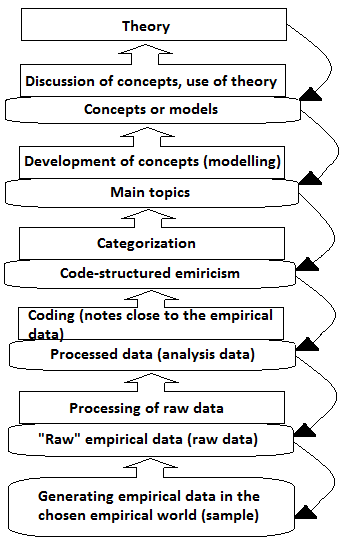
\includegraphics[scale=0.8]{sdi}
\caption[Stepwise deductive inductive method (SDI)]{Stepwise deductive inductive method (SDI) (modified from \cite{tjora})}
\label{fig:sdi}
\end{figure}

As a first step in this model there is data generation and processing of data. In this project we have by hand transcribed every detail from both audio and video recordings from both workshops. This forms the analysing data. We ended up with a huge amount of analysing data constituting for over 25 000 words from workshop 1 and about 6 000 words from workshop 2. The next step from here is coding of this data, which means to put empirical notes on interesting findings. The codes can be words and phrases describing interesting parts of the data material. The point is to try to reuse the codes if they fit to other parts of the findings, or to come up with new codes when new, interesting findings are discovered. After finishing through all the data material, you end up with a set of codes. The codes should only be developed from the empirical data, and not a priori, and it should be a natural link between the set of codes and the data material. In this project we did the coding by putting colors on the different areas in the material that had the same codes. From workshop 1 we handled the transcribed audio and video recordings equally and ended up with 88 codes. From workshop 2 we did the same, and ended up with 44 codes.

Usually, from a large data set you get too many codes to structure the data analysis properly. The next step is therefore to categorise the codes. This means to gather the relevant codes in groups. Here it is the research questions (problemstillingen) which lies in ground for what is relevant. The categories will usually be the main topics for the research's results. From workshop 1, we narrowed it down to 8 main topics, and this is the way we have presented the results in our report. This can be found in Chapter 11. From workshop 2, we ended up with 5 main topics, which are discussed in Chapter 14.

All the work that has been done up to this point has been done with the empirical data as a basis. The next step in the method is to develop concepts. Here theories will be more important. The categories, or main topics, that were developed in the last step, will now be related to theories about the topic. In this project we will set the categories up with the relevant topics discussed in earlier chapters, and use this to come up with a video game concept for elderly. Tjora \cite{tjora} distinguish between concepts and theories. He defines a theory like this (directly translated from Norwegian): "For a concept to have status as a theory, it has to be falsifiable and verifiable" \cite{tjora}. However, development of theories is not something that is done in all research, and it is quite common to use the concepts as legitimate results. In some type of research setting up the main topics or categories and discussion of these, can also be accepted as publishable results. This is what we have done in this study. 

\section{Quality of Research}
\label{sec:qualityresearch}
It is important to evaluate the quality of the research. As discussed earlier in this chapter we would want to maximise three criteria when doing research: generalizability, precision and realism. In our study we are trying to maximie realism, more than the other criteria. In addition there are other criteria that need to be considered when evaluating the quality of research. In \cite{tjora} Tjora discuss the three criteria: \emph{Reliability}, \emph{validity} and \emph{generalizability}. In addition, there are some possible pitfalls when doing qualitative research that needs to be acknowledged. We will discuss these elements in the next sections, and further discuss the quality of our research in Chapter Discussion.  

\subsection{Reliability}
It is important to distinguish between what is data from the research and what is the researcher's own analysis. By using direct citation the reliability of the research will be strengthened. How the informants have been chosen, and the relationship between the researcher and the informants, are important aspects for the reliability. Tjora also discuss the researcher's role in the study, which should idealistically be neutral. However this is impossible to maintain and it is therefore important to discuss how the researcher's position in the study can have an impact on the result \cite{tjora}.

\subsection{Validity}
"Is what we have found the answers to the questions we were actually trying to answer?", is a relevant question when evaluating the validity. In \cite{tjora} Tjora talks about communicative and pragmatic validity. The former gets tested with the research environment, where we relate the research to relevant theories and to previous studies done within the same topic. The latter can be tested with the question on if the research lead to changes or enhancements. The former is the one we primarily care about in the type of research we have done and other types of social science research. The validity will be even more strengthened by being open about how the research is performed and by explaining why certain data gathering methods have been used and the reasons for theoretical input. 

\subsection{Generalizability}
Some type of generalizability is a goal for most research. Tjora presents three kinds of generalizability within qualitative research \cite{tjora}: \emph{naturalistic generalizability}, \emph{moderate generalizability}, and \emph{conceptual generalizability}. The first one is when the researcher describes the details that has been done in the study so good that the reader of the study can self evaluate whether the findings are valid for the his or her own research. The second is about the researcher describing in what type of settings the findings will be valid. Examples of this can be at what time, at what places, in what context etc.. The last one, and also the one Tjora expresses his interest over, is about developing concepts, typologies, or theories that also can be relevant for other cases than the ones being studied. One of the reasons why Tjora has his interests in the last form for generalizing is because this relates to the goal of the SDI-model. In this study we have studied elderly's interactions with commercial video games with a goal of finding what aspects are important when developing a game for this user group. In addition we have studied their attitudes about exercising, and technology in general. The findings done in particular workshop 1, can be relevant also for others working with elderly and technology. Therefore, the third kind of generalizability is relevant in this study.


\subsection{Other quality aspects to consider}
In addition to the three main criteria Tjora also discusses the importance of transparency \cite{tjora}. The goal about this is that the readers should get   good enough insight into the research so that they can self evaluate the quality of the research. Thus, transparency is about presenting and discussing questions like for example how the research has been conducted, the different choices that have been made, what kind of problems that arose etc.. We will discuss this in Section \ref{sec:discQuality}. In addition to the criteria presented by Tjora, we have looked into some issues discussed by Myers and Newman \cite{interview}. They summarise a set of possible pitfalls when doing qualitative research, and in particular when doing qualitative interviews \cite{interview}: \emph{artificiality of the interview}, \emph{lack of trust}, \emph{lack of time}, \emph{level of entry}, \emph{constructing knowledge}, \emph{ambiguity of language}, \emph{elite bias}, \emph{Hawthorne effects} and \emph{interviews can go wrong}. As the topics for our two focus group interviews were more about experience rather than knowledge, and because we did not experience any time pressure, we have evaluated most of these aspects to not have affected our data gathering. The only two of these aspects that might have affected out data gathering are \emph{elite bias} and \emph{Hawthorne effects}. The first is about how the interview can give incomplete and under-representative data  if only one type of group is interviewed, and that it therefore can be hard to understand the broader situation. Because of an overall time limit (the time allocated to the master thesis) and practical reasons, we only included one group of people with the same interests for learning and keeping up with technology. Our data gathering would probably be different, if we gathered a group of "random" people, because they would have different backgrounds and interests. The latter is, as briefly mentioned in Section 8.2.2, that people may behave differently when they are put in a specific setting with researchers interviewing or observing them. These two aspects will also be discussed in more detail in Section \ref{sec:discQuality}.


\section{Recruitment of Participants for the Workshops}
In this study we wanted to involve the relevant user group for the exergame. The relevant user group is senior males and females, aged 65 years and over. Because of time and practical limitations, we contacted an already established group, called "Seniornett". "Seniornett" is an organization in Norway which works to include the older generation (55 years +) in the emerging information technology and to help them gain digital competence. The organization was started in 1997 and is represented in every county in Norway.  Every semester the local clubs arrange 3-4 meetings with different topics related to technology, as well as an one-hour weekly meeting with technology assistance \cite{seniornett}. Even though this group includes seniors who are interested in learning about new technology, which is not common for every senior, we decided that this was a natural place to start recruiting for our workshop. This group may still have the same physical limitations, but may have a higher understanding of technology than other seniors. 

We contacted the manager of the club in Trondheim and briefed him about our project. He invited us to present the topic of our master thesis in their next meeting, which was 25. February 2013. This presentation would both serve as a contribution to this organisation, as well as a promotion of our project. The latter was mostly to gain interest in participating in the planned workshop. The presentation was mainly about the evolution of computer and video games from the beginning until today. As a part of this, we provided a presentation of serious games, and in particular exercise games. We also had a demonstration where we played Kinect Sports 2, shown on a big canvas. We played tennis with only one player, and showed them the possibility of multi-play by playing two players on the skiing game. Since the main topics for the presentation we held for "Seniornett" are not the main interest in this thesis, we will nor discuss the presentation any further. However, the presentation slides can be found in Appendix XXX for the interested reader. 

After the demonstration and the following discussion, we presented the planned workshop and invited the audience to help us with this. We told them that to make a user-friendly game, it is very important to involve the user, and that their help would mean a lot for our work on developing a game concept. We also explained what was expected from the participants in the workshop, and that this would be video- and audio recorded. In addition, we informed them that participating is voluntary and that the project is legally reported to \ac{nsd}. Everyone in the audience got a document containing information about the project and inform consent, see Appendix Y. Four people signed up at that time. 4 people signed up later by e-mail.

During and after the presentation the audience had some comments and questions. This feedback will be taken into account in our further work, but for convenience, we will discuss them together with the findings from workshop 1. 

\section{Execution of Workshop 1}
\label{sec:ws1}
We will now describe the set up and the execution of workshop 1. We will describe the purpose of the workshop, provide general information about participants, location and equipment, and present how the workshop was set up and performed. 

The primary goal for our first workshop was to introduce the participants, from now on called informants, to the Xbox Kinect technology and to three commercial games. We wanted to observe how they interacted with the technology and how well they enjoyed playing. In addition we had a focus group interview where the informants could talk about how they experienced the gaming session. We also used a short survey to get to know the informants' technology experience and attitude towards exercising.   

\subsection{General information}
The workshop was held over a two day period, the 13th and 14th of March, with location at "Gulhuset, Voll gård", a place familiar to the informants from "Seniornett". The workshop started around 2 pm and lasted approximately three hours. We had recruited eight informants from "Seniornett" to our workshop, three males and five females. They were divided into two groups, one for each day. One of the recruited females had an accident, which made it difficult for her to participate in the workshop. We therefore ended up with seven informants. The informants average age was 70.6 years (with a standard deviation of 7,9 years). In addition to us and the informants, we had two Ph.D. students with us the first day who acted in the role as facilitators. The second day our supervisor, Lill Kristiansen, joined us and took the role as the facilitator.   

In advance we had sat up an agenda for how we wanted to carry out the two workshop days,  see Table \ref{tab:agendaW1}.  

\begin{table} [ht!]
\centering
    \begin{tabular}{|l|l|}
       \hline
       \textbf{Introduction} & 15 minutes  \\ \hline
       \textbf{Survey} & 10 minutes  \\ \hline
       \textbf{Single play} & 15 minutes for each participant \\ \hline
       \textbf{Multi play} & 10 minutes for each participant \\ \hline
	   \textbf{Group discussion} & 65 minutes \\ \hline
    \end{tabular}
    \caption[Workshop Agenda]{Workshop agenda}
    \label{tab:agendaW1}
\end{table}  

\subsubsection{Location and Equipment}
We used "Gulhuset, Voll gård" as location for our workshop, because it is a location well known for the informants. This location is used for various events, like theme lectures, song meetings, and story telling gatherings, and has couches, tables and chairs, and a small kitchen where it is possible to make coffee and something to eat. "Gulhuset" was ideal to use for our workshop, not only because is is familiar to the informants, but because it was possible to make a living room-like atmosphere. It was also ideal because it is a place where we imagine that elderly could meet and play a future exercise game. At "Gulhuset" also possess a screen and a projector, which we used for our introduction. However, during the gaming session we chose to use a 46" Samsung flat screen. This was to make the gaming experience as natural as possible, as most people do not have screens and projectors in their own homes. We borrowed the flat screen from our department at NTNU. In addition to the the flat screen we had a Xbox, a Kinect sensor and three commercial games, which where use for the gaming session. This equipment was bought with support from a foundation for master thesis with computer science as subject [ENDRE litt på denne].   

In the workshop we used both video and audio recording to be able to interact with the informants. We rented a dictaphone, two video cameras (a Sony Handycam and a Panasonic 3MOS) and a rack for each camera. We wanted to use two video cameras to be able to make recordings from different angles. We had one video camera in the front of the room to capture movement and facial expressions, and we had one in the back to see movements from behind, in addition to recording interaction with the Kinect sensor and the games. The dictaphone was used for the group discussion.    

\subsection{Chosen games}
We spend some time looking through different types of games to find suitable games for the workshop. We evaluated the different games by reading reviews, looking at videos on YouTube and trying some free demos online. We chose three different commercial games: \emph{Fruit Ninja}, \emph{Your Shape Fitness Evolved 2012}, and \emph{Kinect Sports Season Two}. These games all provides some different properties that we found important for our study.  

\subsubsection{Fruit Ninja}
"Fruit Ninja" is a game where you have to use your arms like a ninja to slice fruit that is thrown up into the air. The goal is to slice as much fruit as possible in a short period of time, without hitting any bombs that are thrown up together with the fruit. This games features simultaneous multi play with both competition and cooperation. Figure \ref{fig:fruitninja} shows a screen-shot from the game where two players cooperate to slice as much fruit as possible. The reason for why we chose to use Fruit Ninja in the workshop was to present the informants for a game based on pure fun and movement, with a concept far from something one might experience in real life. 

\begin{figure} [H]
\centering
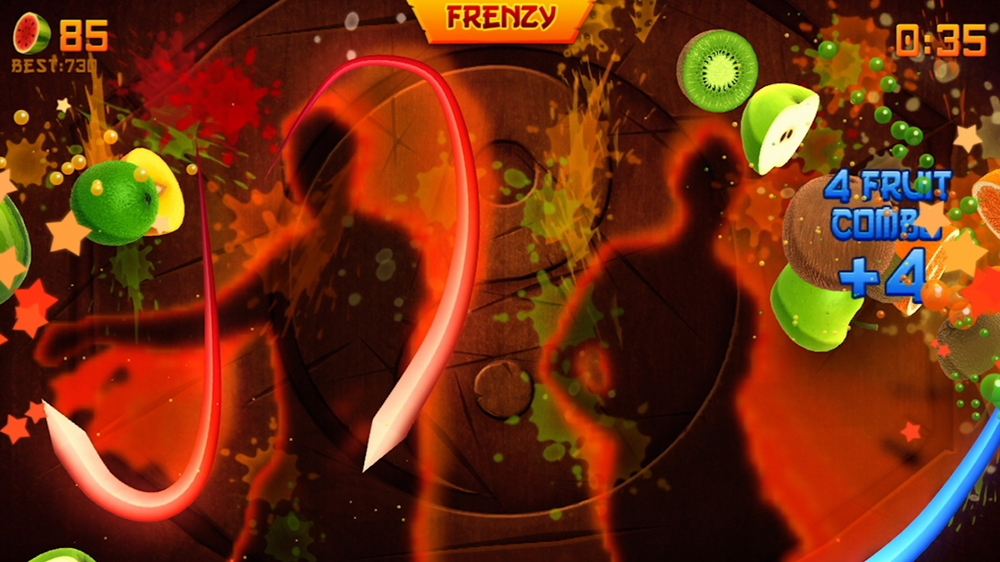
\includegraphics[scale=0.4]{fruitninja}
\caption[Fruit Ninja Multi-Play]{A screen-shot of two players playing "Fruit Ninja" together \cite{fruitninja}}
\label{fig:fruitninja}
\end{figure}

\subsubsection{Your Shape Fitness Evolved 2012}
"Your Shape Fitness Evolved 2012" is a popular exercise game for Kinect. This game has over 90 hours of activities, which can be used to design your own workout program. \emph{Your Shape Fitness Evolved 2012} follows your shape, fitness level and goals, and uses this to schedule the difficulty for the activities. You have the possibility to choose exercises for specific muscle groups, you can join classes like jump rope, cardio boxing and yoga, or you can take a virtual run in New York or Paris \cite{yourshape}. In addition, Your Shape Fitness Evolved provide three Humana-sponsored \footnote{Humana is a health care provider, see http://www.humana.com/ for details.} exercising games. These games are aimed to encourage fitness for two specific age groups: kids and elderly. In addition, it has a program to reduce high blood-pressure and strengthen the heart \cite{ptspill}. We chose to use the Humana game "Aging with Grace" to present a program that is specifically designed for elderly. This game is designed with exercise as the main purpose, and provide different aerobic movements. A virtual personal trainer shows the player how to do the exercises and offers real-time feedback. In Figure \ref{fig:ptspill} you can see a picture from "Aging with Grace", where the player (to the right) performs step touch together with the virtual trainer (to the left). 

\begin{figure} [H]
\centering
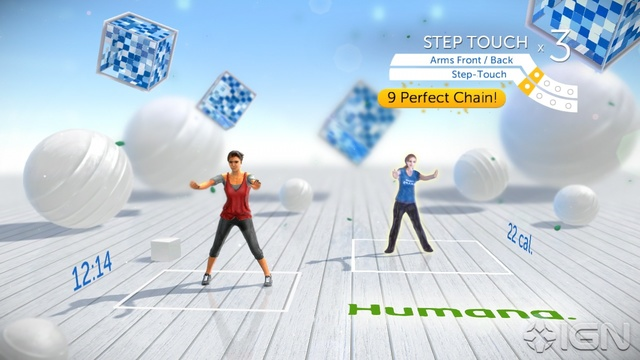
\includegraphics[scale=0.5]{ptspill}
\caption[Your Shape Fitness Evolved 2012]{A screenshot from a Humana-sponsored game in "Your Shape Fitness Evolved 2012" \cite{ptspill}}
\label{fig:ptspill}
\end{figure}

\subsubsection{Kinect Sports: Season Two}
"Kinect Sports: Season Two" is a game that consist of a bundle of six sports, which are tennis, darts, base ball, American football, skiing and golf. These sports stimulates movement and activity in a fun and motivating way, though exercise is not the main focus. "Kinect Sports: Season Two", depending on the sport chosen, offers both competitive and cooperative multi-play. Figure \ref{fig:sportsgame} show the two chosen games: skiing and tennis. Figure \ref{fig:elderlyskii} shows to informants playing the skiing game together. We wanted to present this game for the elderly because of its amusing and real-life activities. 

\begin{figure} [H]
\centering
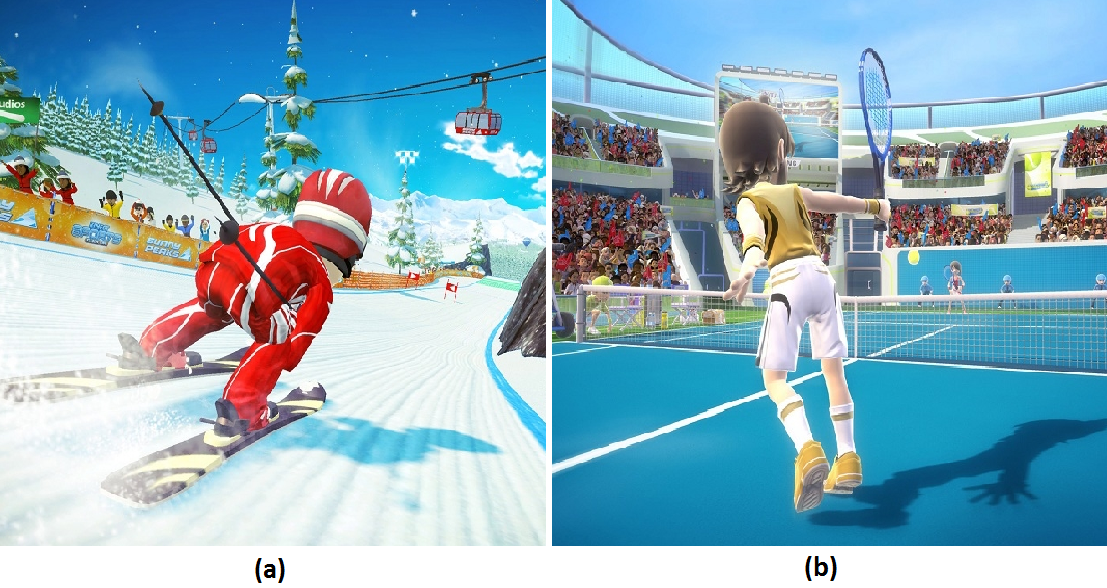
\includegraphics[scale=0.45]{skiitennis}
\caption[Kinect Sports Season Two, Skiing and Tennis]{A screenshot from (a) skiing, and (b) tennis in "Kinect Sports: Season Two" \cite{sportsgame}}
\label{fig:sportsgame}
\end{figure}

\begin{figure}
\centering
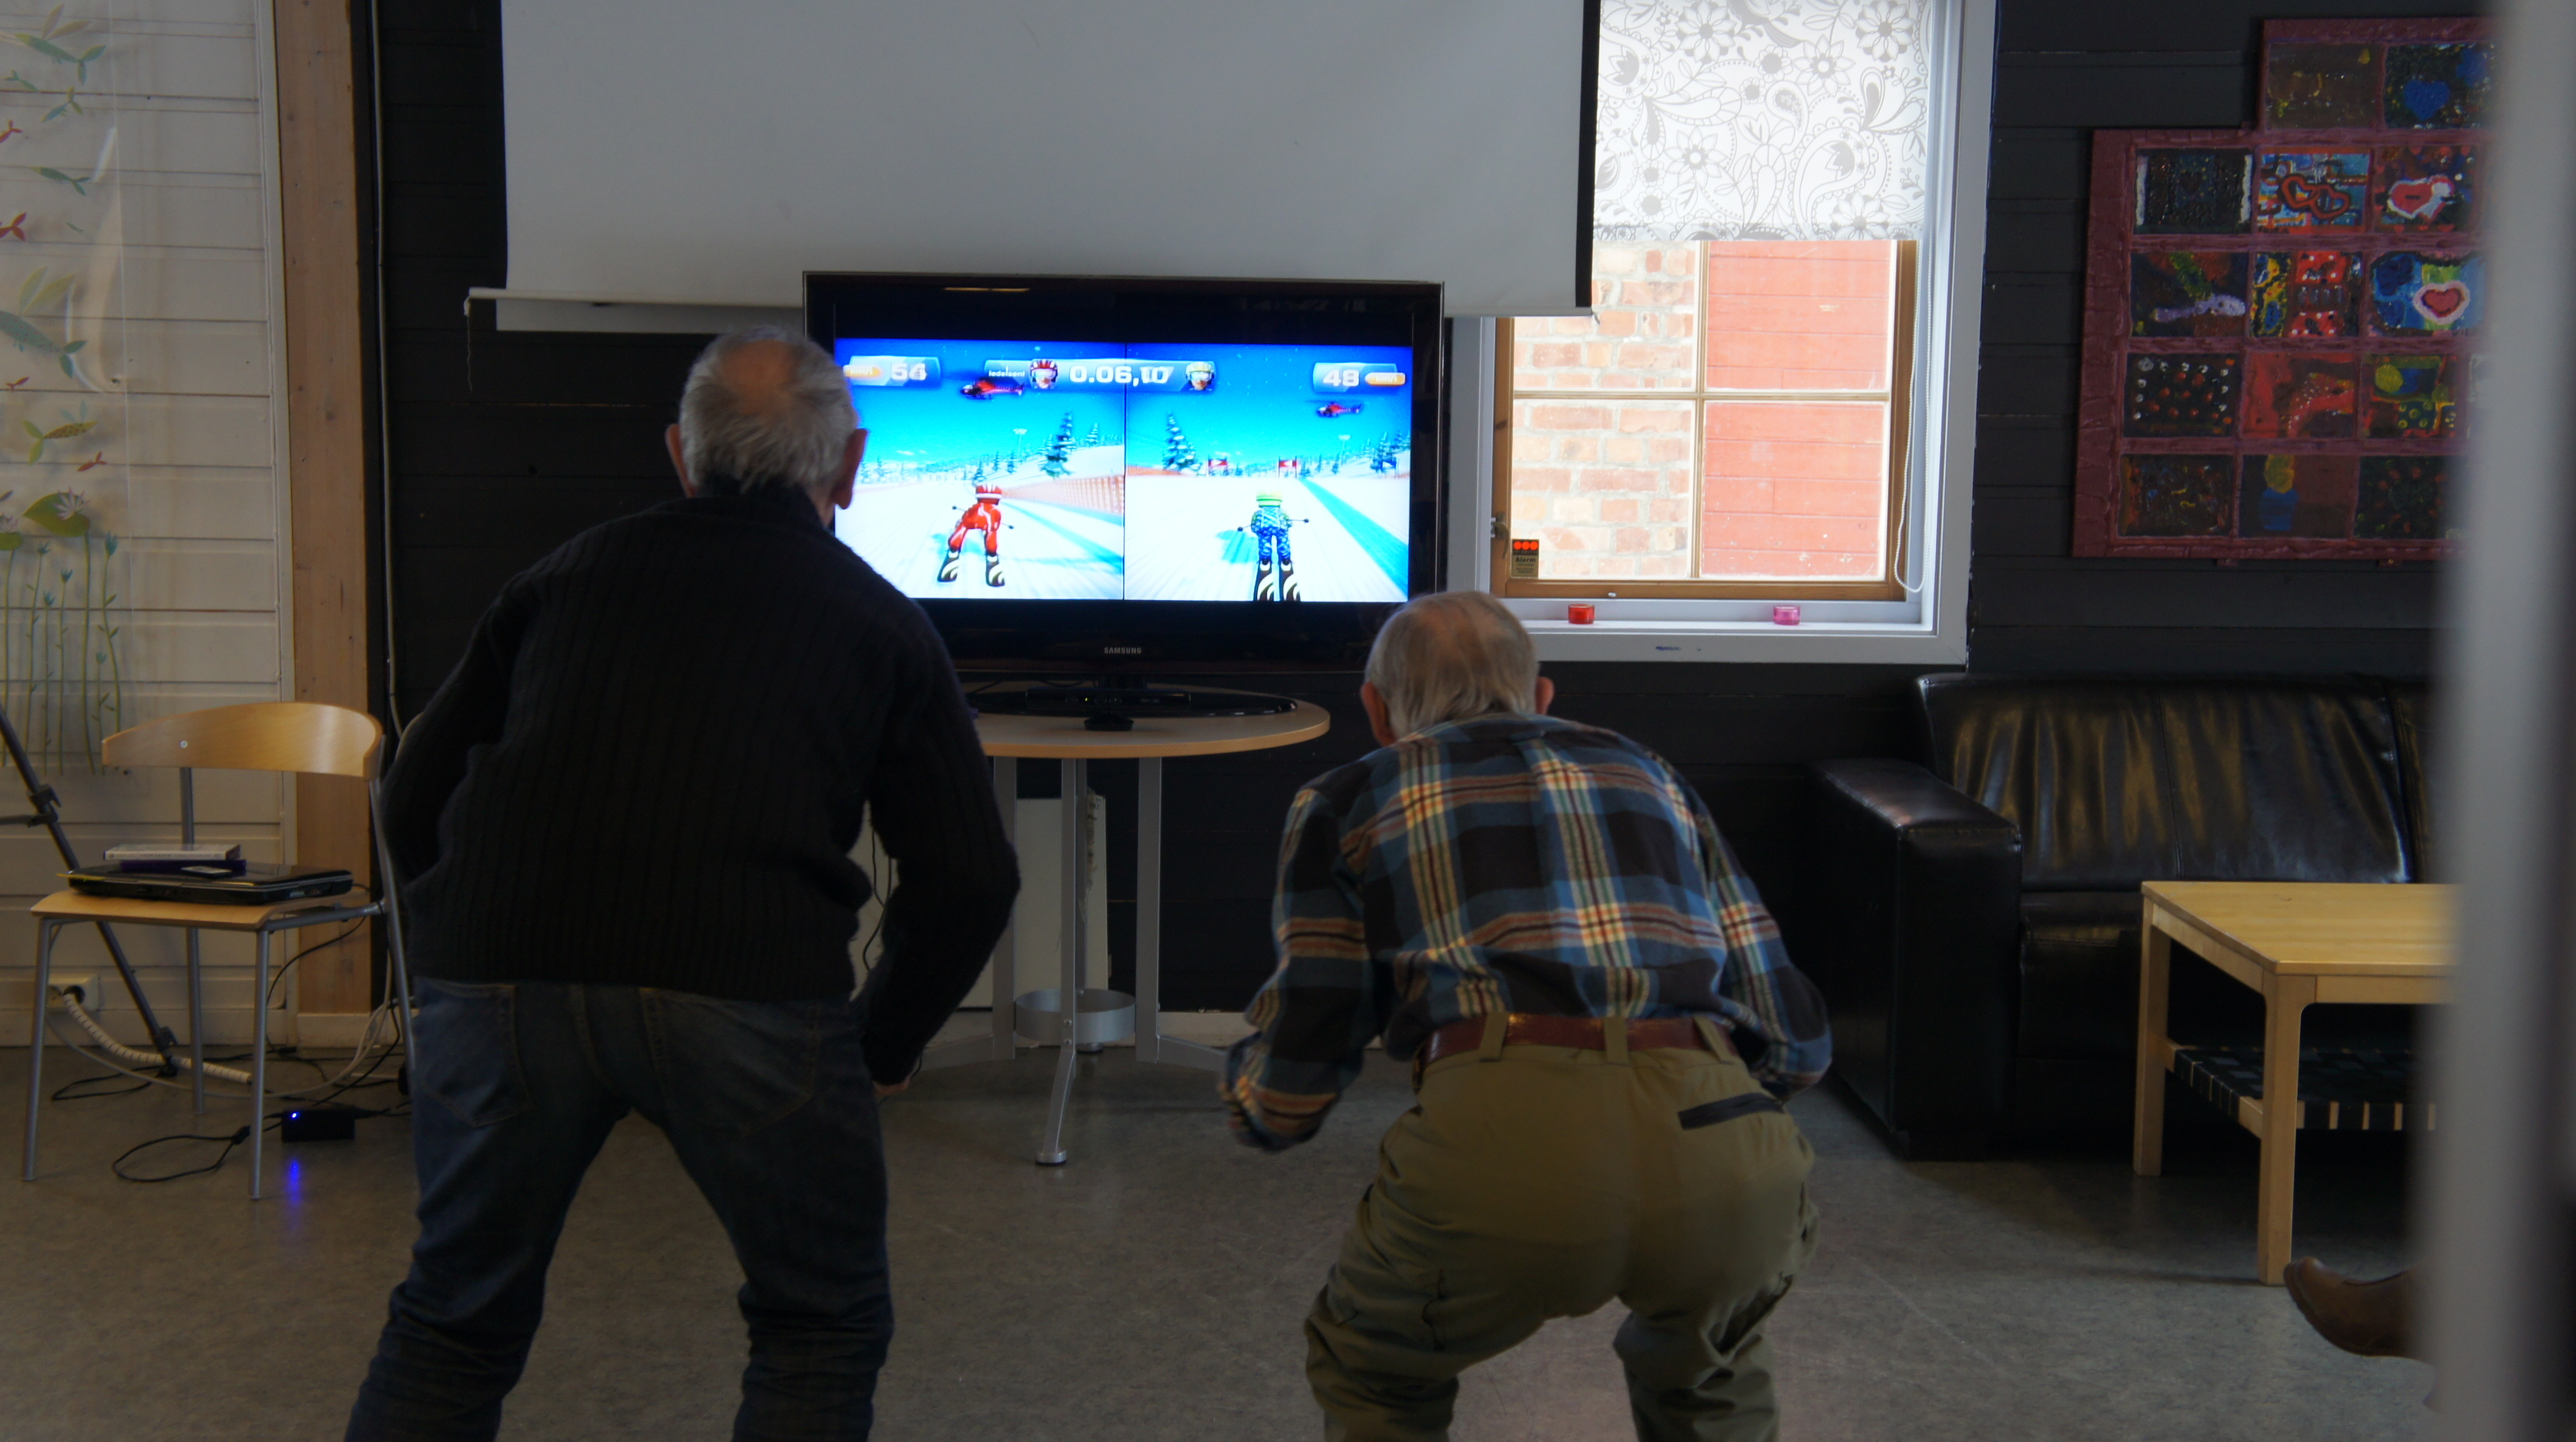
\includegraphics[scale=0.5]{eldreSpiller.jpg}
\caption[Kinect Sports Season Two, Multi-play]{Two informants compete in the skiing game offered in Kinect Sports: Season Two}
\label{fig:elderlyskii}
\end{figure}

\subsection{Execution}
In the introduction we shortly presented ourselves and the background and main goal for our master thesis. We also informed about the purpose of the workshop, and presented the agenda for the day. The main part of the introduction was a review of the consent form, see Appendix X, where we highlighted important aspects as video and audio recording and that participation is voluntary. After the introduction the informants had some time to look over the consent form before they signed two copies, one for themselves and one for us. We then handed out a short survey to the informants, where they were asked a few questions about themselves, their technology experience and their attitudes towards exercising. 

After finishing this session we started the gaming. The gaming session was divided into two parts, one part where the informants played games individually, and one where they played together in pairs. The order of which part that where played first was for randomisation changed from day one to day two. In workshop day one there were only three informants, so they took turns playing during the multi player part. "Your Shape Fitness Evolved 2012" and tennis from "Kinect Sports: Season Two" were used for single play, while "Fruit Ninja" and skiing from "Kinect Sports: Season Two" were used for multi play. 

Initially we wanted to start the play session without us helping the informants. We wanted to observe how well the informants understood the technology and the games presented for them. We believed that this would give us a more realistic result. We started out like this on day one of workshop 1 However, we experienced that the informants had problems understanding what they were suppose to do which lead to frustration and a bad experience. Therefore, after finishing the individual games, and before starting the multi player session, we explained how the Kinect sensor works and showed how to interact with the sensor. We also described the games they where about to play, and the goal of the games. On day two of workshop 1 we started with multi player and gave them the same introduction to the technology as before the multi player session on day one. On the games where they played individually, they went through the menu themselves on both day one and two. We guided them when necessary. 

When the informants had played individually and together in pairs we had a focus group interview. We asked them open questions about their experience of the technology and the gaming session. We wanted to know if they liked the games or not, and if so why. It was also in our interest to find out if this technology was something the informants would use, and if they could imagine using it for exercise. Our questions from our interview guide served just as a starting point for discussion, most of the time the informants talked freely with us and each other. The interview guide can be found in Appendix ..                 


\section{Execution of Workshop 2}
\label{sec:ws2}
We will now describe the set up and the execution of workshop 2. We will describe the purpose of the workshop, provide general information about participants, location and equipment, and present how the workshop was set up and performed. 

The aim of workshop 2 was to involve the target user group in the development process. We invited all the informants that participated in workshop 1 to a second workshop where we wanted to present our prototyped video game concept. The reason for inviting the informants to this second workshop was to get feedback on the prototypes, which is highly valuable when creating a user-friendly video game for elderly. This group of informants represents in this case the group of elderly that this game is targeted for, and are potentially future users of the system. They know know the interests and needs for this user group. In this workshop, we tried to give the informants an realistic impression of what an exercise game, based on their feedback, would look like. The way we presented the game was by prototypes made from PowerPoint and Photoshop. These are tools that were familiar to us, and it did not require any extra time to learn how to use them. Since we were in an early stage of the development process of a potential exergame, we focused on using low-cost prototypes.  

\subsection{General information}
Workshop 2 was held the 25th of April at "Gulhuset, Voll gård", the same location used for workshop 1. We met around 1 pm and started our presentation 20 minutes later. The total duration for workshop 2 was approximately two hours. We invited all the participants from workshop 1. Four informants chose to participate in workshop 2, in addition to the one women that was hindered to attend workshop 1 due to an accident. The group consisted of three men and two women. The informants average age was ... (with a standard deviation of ... years). We did not have any additional facilitators at this workshop. 

Beforehand, we had sat up this agenda:

\begin{itemize}
\renewcommand{\labelitemi}{$\bullet$}
\item Welcome.
\item Practical information.
\item Findings from workshop 1.
\item Presentation of our video game concept.
\item Feedback on our video game concept.
\item Presentation of our menu proposal.
\item Feedback our menu proposal.
\item Summary and finish.
\end{itemize}


\subsubsection{Location and Equipment}
We used the same premises as in workshop 1: "Gulhuset, Voll gård". 
For this presentation we only needed a laptop, a projector, and a screen. We used a private laptop, and the premises' screen and projector. Because of our desire to give our full attention to the presentation and discussion, we also video recorded this workshop. This was done with the use of a video camera, because we wanted to capture facial expressions in addition to the oral feedback. The video camera was a Panasonic 3MOS, and was borrowed from our department at NTNU. To make a cosy and comfortable atmosphere, we served cake and coffee.   

\subsection{Execution}
We started the presentation with an introduction, presenting ourselves, the goal of the workshop, and the agenda for the next hours. Some practical information about duration, the video recording, and requirements due to anonymity were also presented. The a short summary of workshop 1 was given, as well as the most important findings from this workshop. We did this both to fresh up the informants' memory, and to give the new informant a recap of workshop 1. This was also done to give the informants an idea of what we have focused on when creating our video game concept.        

In this workshop we alternated between presentation and discussion, so that there should not be too much information to remember for the informants. First, we presented the overall idea for the concept, before we proceeded with a more detailed description of the video game. The video game series was presented. We showed them prototypes of two different games from this series. We presented the games one by one, with an individual group discussion for each of them. To make it easier for the informants to comment and discuss we handed out pictures of the prototyped scenes (Sette inn figur/bilde av bilder på bord). 

We also presented for the informants the menu prototype we had made. We tried to present the menu in a way to make it look as realistic to a Kinect video game as possible. One of us stood in front of the screen simulating game play by pretending to "push the buttons", while the other controlled the PowerPoint presentation.  After the menu presentation we opened for a new, and final, group discussion. 

After the final group discussion was over, we took a few minutes to greet the informants, and thank them for their feedback, time, and participation.
 

